\chapter[Random Integers and the Poisson Dirichlet Law]{Random Integers, the Poisson Dirichlet Law\\ and Chebotarev as a Dirichlet Process}\label{ch:pd}

Chapter~\ref{ch:recip} built a Gamma process from the prime factors of a zeta distributed random integer, and Chapter~\ref{ch:hit} computed the laws of the labels of its largest prime factors. Both are known objects under other names, some of which Chapter~\ref{ch:recip} recalled (Billingsley, Lloyd \cite{lloyd1984}), and this chapter develops them. The normalised sizes of the prime factors of a random integer converge to the Poisson Dirichlet law with parameter $1$, the limit law of the normalised cycle lengths of a uniform random permutation (Billingsley; Donnelly and Grimmett; Arratia, Barbour and Tavar\'e); the share of the largest prime factor follows Dickman's law; the number of prime factors is asymptotically normal by the theorem of Erd\H{o}s and Kac; and the Gamma process of Chapter~\ref{ch:recip}, normalised, is Ferguson's Dirichlet process. Chebotarev's theorem, in its Dirichlet density form, is then the statement that the base measure is Haar measure, and the limits of the Frobenius functionals of Chapter~\ref{ch:recip} are a standard exponential variable times a Dirichlet mean, so that the Gamma times Dirichlet mean factorisation of James, Roynette and Yor, whose atomic case is Theorem~\ref{thm:lapspline}, and Theorem~\ref{thm:recipggcfun} describe the same laws.

The results are of three kinds, and the Notes say which are known. Theorem~\ref{thm:pddirichlet} extends the Dirichlet law of the shares of Chapter~\ref{ch:recip} to the Dirichlet process limit and identifies the limit of a Frobenius functional as a standard exponential variable times a Dirichlet mean. Theorem~\ref{thm:pdtheta} shows that for the random integers weighted by the coefficients of $\zeta^\vartheta$, the ones that drive the zeta subordinator of Chapter~\ref{ch:10d}, the normalised sizes of the prime factors converge to the Poisson Dirichlet law with parameter $\vartheta$, so that powers of $\zeta$ give the whole Ewens family. Theorem~\ref{thm:pdmertens} gives the rates at which three natural colourings of the prime factors of a uniform random integer below $x$ approach Haar measure: the largest factor faster than any power of $1/\log x$ (Dawsey's theorem), the size biased factor at rate $1/\log x$, and the count of distinct factors only at rate $1/\log\log x$, the last two with explicit constants which are Mertens constants per Chebotarev class. The last rate shows in the data: among the distinct prime factors of random integers below $10^7$, the identity class of $S_3$ for $x^3-x-1$ accounts for $7.2$ percent of them against its Haar measure of $16.7$ percent, because no prime below $59$ lies in that class. Section~\ref{sec:pdprogress} then answers two questions and bounds a third from one side: the Mertens constants per class are explicit in $L(1,\chi)$ and $\frac{L'}L(1,\chi)$ (Theorem~\ref{thm:pdmertensL}); for an Euler product whose logarithm has nonnegative coefficients, given at the primes by a continuous function of equidistributed labels, the Ewens parameter is the exponent of the singularity at $s=1$ (the order of the pole when there is one), and the colouring of its random integer is the equidistribution measure weighted by that function (Theorem~\ref{thm:pdewens}); and in the Kolmogorov distance of the shares the Dirichlet process limit is approached no faster than $(\sigma-1)^{\delta_{\min}}$, because the smallest class is empty with probability of that order, which Chapter~\ref{ch:recip} found and Theorem~\ref{thm:pdrate} gives with its constant.

\section{The Poisson Dirichlet law}\label{sec:pdlaw}

Let $U_1,U_2,\dots$ be independent uniform variables on $(0,1)$ and define the stick breaking sequence $W_1=U_1$, $W_k=(1-U_1)\cdots(1-U_{k-1})U_k$. The sequence $(W_k)$ sums to $1$; its decreasing rearrangement $V_1\ge V_2\ge\dots$ has the \emph{Poisson Dirichlet law} $\mathrm{PD}(1)$, and $(W_k)$ itself is its size biased permutation, the GEM law \cite{kingman1993,pitman2006}. Two descriptions matter here. First, if $\Gamma$ is a standard Gamma subordinator on $[0,1]$, with L\'evy measure $x^{-1}e^{-x}dx$, then the ranked jumps of $\Gamma$ divided by $\Gamma(1)$ have the law $\mathrm{PD}(1)$ \cite{kingman1975}, and the quotient is independent of $\Gamma(1)$, which is standard exponential. Second, if $\pi_n$ is a uniform random permutation of $n$ letters, the ranked cycle lengths divided by $n$ converge in law to $\mathrm{PD}(1)$, a fact that goes back to Shepp and Lloyd \cite{shepplloyd1966}. Its analogue for prime factorisations is Billingsley's theorem \cite{billingsley1972}, found independently by Knuth and Trabb Pardo \cite{knuthtrabbpardo1976}; Donnelly and Grimmett \cite{donnellygrimmett1993} gave a short proof by size biased sampling, and Arratia, Barbour and Tavar\'e \cite{arratiabarbourtavare2003} treat integers and permutations together as logarithmic combinatorial structures.

\begin{theorem}[Billingsley \cite{billingsley1972}]\label{thm:pdbillingsley}
Let $n$ be uniform on $\{2,\dots,x\}$ with prime factorisation $n=\prod p_i^{e_i}$, and let $V_1(n)\ge V_2(n)\ge\dots$ be the decreasing rearrangement of the numbers $e_i\log p_i/\log n$, padded with zeros. As $x\to\infty$, $(V_1(n),V_2(n),\dots)$ converges in law to $\mathrm{PD}(1)$. In particular $\log P^+(n)/\log n$, with $P^+$ the largest prime factor, converges in law to $V_1$, whose distribution function is Dickman's function \cite{dickman1930}, $\Prob(V_1\le v)=\varrho(1/v)$, where $\varrho(u)=1$ on $[0,1]$ and $u\varrho'(u)=-\varrho(u-1)$ for $u>1$; its mean is the Golomb Dickman constant $0.62433$.
\end{theorem}

The parameter $1$ is the order of the pole of $\zeta$ at $s=1$, and the error in the convergence is at most of order $1/\log x$ (Tenenbaum \cite{tenenbaum2000}). The number of prime factors has its own limit law.

\begin{theorem}[Erd\H{o}s and Kac; Sathe and Selberg]\label{thm:pderdoskac}
Let $\omega(n)$ be the number of distinct prime factors of $n$ uniform on $\{1,\dots,x\}$. Then $(\omega(n)-\log\log x)/\sqrt{\log\log x}$ converges in law to the standard normal law \cite{erdoskac1940}. More precisely \cite{sathe1953,selberg1954}, uniformly for $1\le k\le A\log\log x$, for any fixed $A>0$,
\[
\Prob(\omega(n)=k)=\frac{(\log\log x)^{k-1}}{(k-1)!\,\log x}\Bigl(G\Bigl(\frac{k-1}{\log\log x}\Bigr)+O\Bigl(\frac1{\log\log x}\Bigr)\Bigr),
\]
where
\[
G(z)=\frac1{\Gamma(1+z)}\prod_p\Bigl(1+\frac z{p-1}\Bigr)\Bigl(1-\frac1p\Bigr)^z,
\]
and $\E\,\omega(n)=\log\log x+B+O(1/\log x)$ with $B=0.26150$ the Mertens constant \cite{tenenbaum2015}, while $\operatorname{Var}\omega(n)=\log\log x+B-\frac{\pi^2}6-\sum_pp^{-2}+o(1)$ (Diaconis, Mosteller and Onishi \cite{diaconismostelleronishi1977}).
\end{theorem}

Figure~\ref{fig:pdintegers} shows both theorems at $x=10^7$ for $400000$ random integers, factorised with a sieve of smallest prime factors. The empirical distribution of $\log P^+/\log n$ differs from Dickman's $\varrho(1/v)$ by at most $0.066$, the supremum being approached as $v\uparrow1$, where the $6.6$ percent of integers below $10^7$ that are prime form an atom at share $1$, and this is the $1/\log x$ term with $\log x=16.1$. The mean is $0.6463$ against $0.6243$, and the second largest share has mean $0.2255$ against the $\mathrm{PD}(1)$ value $0.2096$. The mean of $\omega(n)$ is $3.014$, against $\log\log x+B+(\gamma_{\mathrm E}-1)/\log x=3.015$, but the variance is $1.10$, far below the mean (the formula of Theorem~\ref{thm:pderdoskac} without its $o(1)$ term gives $0.94$), and neither the Poisson law with mean $3.04$ nor the normal law of Erd\H{o}s and Kac fits the histogram at this $x$, where $\log\log x=2.78$. The mean of $\Omega(n)-\omega(n)$, which counts repeated factors, is $0.7723$ against $\sum_p1/(p(p-1))=0.7732$.

\begin{figure}[!htbp]
\centering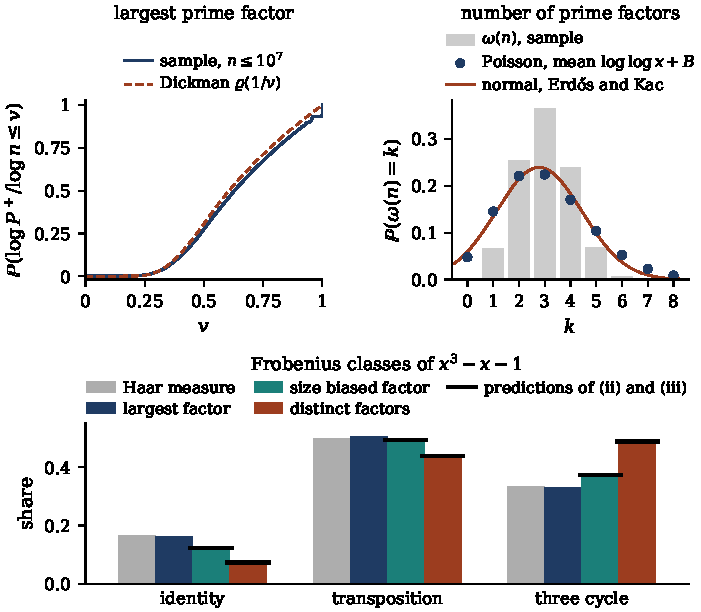
\includegraphics[width=\textwidth]{figs/pd_integers.pdf}
\caption{A sample of $400000$ uniform random integers below $10^7$. Top left: the empirical distribution function of $\log P^+/\log n$ against Dickman's $\varrho(1/v)$ (Theorem~\ref{thm:pdbillingsley}). Top right: the histogram of the number $\omega(n)$ of distinct prime factors, whose mean is close to $\log\log x+B$, with the Poisson law of mean $\log\log x+B$ and the normal law of Erd\H{o}s and Kac, of mean and variance $\log\log x$, neither of which fits at this $x$ (Theorem~\ref{thm:pderdoskac}). Bottom: three colourings of the prime factors by their Frobenius class in the $S_3$ field of $x^3-x-1$ (the class of the largest factor, of a size biased factor, and of the distinct factors pooled over the sample), against Haar measure; the short bars are the predictions of Theorem~\ref{thm:pdmertens}(ii) and (iii) with the constants of Table~\ref{tab:pdmertens}.}\label{fig:pdintegers}
\end{figure}

\section{The Dirichlet process of a random integer}\label{sec:pddirichlet}

Ferguson's Dirichlet process with base measure $\vartheta\mu$, for $\vartheta>0$ and a probability measure $\mu$ on a compact metric space $Y$, is the random probability measure $P=\Gamma_{\vartheta\mu}/\Gamma_{\vartheta\mu}(Y)$ obtained by normalising the Gamma random measure with shape measure $\vartheta\mu$ (\cite{ferguson1973}, Section~4); for every partition $B_1,\dots,B_k$ of $Y$ the vector $(P(B_1),\dots,P(B_k))$ has the Dirichlet law with parameters $(\vartheta\mu(B_1),\dots,\vartheta\mu(B_k))$, and $P$ is independent of the total mass $\Gamma_{\vartheta\mu}(Y)$, which is Gamma with shape $\vartheta$ (\cite{jamesroynetteyor2008}, Section~1.4; \cite{pitman2006}, Section~4.2). Written as $P=\sum_iV_i\delta_{y_i}$ with $V_1\ge V_2\ge\dots$, its weights have the law $\mathrm{PD}(\vartheta)$ and its labels $y_i$ are independent of the weights and of one another, with law $\mu$ (several labels coincide when $\mu$ has atoms); $\mathrm{PD}(1)$ is the case $\vartheta=1$ of Section~\ref{sec:pdlaw}.

Let $N_\sigma$ be the zeta random integer of Chapter~\ref{ch:recip}, $\Prob(N_\sigma=n)=n^{-\sigma}/\zeta(\sigma)$, with prime exponents $e_p$, and let $(\theta_p)$ be labels in $Y$, equidistributed with respect to $\mu$ outside a finite set $S$ of primes. The labelled factorisation is the random measure
\[
\Xi_\sigma=\sum_{p\notin S}(\sigma-1)e_p\log p\;\delta_{\theta_p},
\]
and Theorem~\ref{thm:recipgammaproc} says that $\Xi_\sigma$ converges in law to the Gamma random measure $\Gamma_\mu$ as $\sigma\downarrow1$.

\begin{theorem}[Chebotarev as a Dirichlet process; after \cite{ferguson1973,cifarelliregazzini1990}]\label{thm:pddirichlet}
As $\sigma\downarrow1$:
\begin{enumerate}
\item[(i)] the normalised labelled factorisation $\mathcal P_\sigma=\Xi_\sigma/\Xi_\sigma(Y)$, set equal to $\mu$ on the event $A_\sigma$ that $N_\sigma$ has no prime factor outside $S$, converges in law, as a random probability measure on $Y$ with the weak topology, to the Dirichlet process $P$ with base measure $\mu$, and jointly with it the total mass $\Xi_\sigma(Y)=(\sigma-1)\sum_{p\notin S}e_p\log p$ converges to a standard exponential variable $E$ independent of $P$;
\item[(ii)] for every continuous $Q\ge0$ on $Y$ the Frobenius functional $\Xi_\sigma(Q)$ converges in law to $E\int_YQ\,dP$, a standard exponential variable times a Dirichlet mean, and
\begin{align*}
\E\exp\Bigl(-\lambda\,E\!\int_YQ\,dP\Bigr)&=\E\Bigl(1+\lambda\!\int_YQ\,dP\Bigr)^{-1}\\
&=\exp\Bigl(-\int_Y\log(1+\lambda Q)\,d\mu\Bigr);
\end{align*}
\item[(iii)] for a partition of $Y$ into $\mu$ continuity sets $B_1,\dots,B_k$ with $\mu(B_i)>0$, the shares $\mathcal P_\sigma(B_i)$ converge jointly in law to the Dirichlet law with parameters $\mu(B_i)$, so that each share $\mathcal P_\sigma(B)$ converges to a Beta variable with parameters $(\mu(B),1-\mu(B))$, of mean $\mu(B)$.
\end{enumerate}
\end{theorem}

\begin{proof}
(i) The map $\xi\mapsto(\xi/\xi(Y),\xi(Y))$ is continuous, in the weak topology, at every finite measure with $\xi(Y)>0$, a set of full $\Gamma_\mu$ probability, so the continuous mapping theorem and Theorem~\ref{thm:recipgammaproc}(ii) give convergence of $(\mathcal P_\sigma,\Xi_\sigma(Y))$ to $(\Gamma_\mu/\Gamma_\mu(Y),\Gamma_\mu(Y))$, which is Ferguson's construction of the Dirichlet process with base measure $\mu$, independent of the Gamma total mass of shape $\mu(Y)=1$. (ii) $\Xi_\sigma(Q)=\Xi_\sigma(Y)\int Q\,d\mathcal P_\sigma$ converges by (i) to $E\int Q\,dP$. The first equality is the Gamma integral $\E e^{-\lambda Em}=(1+\lambda m)^{-1}$, conditioned on $\int Q\,dP=m$ and using independence; the second is Theorem~\ref{thm:recipggcfun}, since $\Xi_\sigma(Q)$ converges in law to the GGC whose Laplace transform is the right hand side. (iii) follows from (i): $\E P(\partial B_i)=\mu(\partial B_i)=0$, so $\nu\mapsto(\nu(B_1),\dots,\nu(B_k))$ is continuous at almost every $P$, and the shares of a Dirichlet process are Dirichlet.
\end{proof}

For Frobenius classes in a finite Galois group $G$, with $\mu$ the image of Haar measure on the set of classes, Chebotarev's theorem supplies the hypothesis, and the proof of Lemma~\ref{lem:recipnu} uses only its Dirichlet density form $\sum_{p\in C}(\log p)p^{-s}\sim\delta(C)/(s-1)$ as $s\downarrow1$, with $\delta(C)=|C|/|G|$. Then (i) and (iii) are Corollary~\ref{cor:recipchebgamma}(ii) of Chapter~\ref{ch:recip} read as a statement about the Dirichlet process: the share $\mathcal P_\sigma(C)$ carried by the primes with Frobenius in a class $C$ is asymptotically $\mathrm{Beta}(\delta(C),1-\delta(C))$, with mean Chebotarev's density $\delta(C)$.

The identity between the last two expressions in (ii), $\E(1+\lambda\int Q\,dP)^{-\vartheta}=\exp(-\vartheta\int\log(1+\lambda Q)\,d\mu)$ for a Dirichlet process with base measure $\vartheta\mu$, is Cifarelli and Regazzini's identity for Dirichlet means \cite{cifarelliregazzini1990}, the Markov Krein identity when $\vartheta=1$ (Diaconis and Kemperman \cite{diaconiskemperman1996}), in the form of James, Roynette and Yor (\cite{jamesroynetteyor2008}, Section~1.4, (33)): a GGC of finite Thorin mass is a Gamma variable times an independent Dirichlet mean, whose atomic case, Theorem~\ref{thm:lapspline}, writes atomic Thorin laws as Gamma variables times B spline variables. Here it says what the Thorin measure of a Frobenius functional is: the limit of $\Xi_\sigma(Q)$ is a GGC with Thorin mass $\mu(Q>0)$ and Thorin measure the image of $\mu$ restricted to $\{Q>0\}$ under $1/Q$ (Theorem~\ref{thm:recipggcfun}), and it is also a Gamma variable of shape $\mu(Q>0)$ times the Dirichlet mean $\int Q\,dP'$ of an independent Dirichlet process $P'$ with base measure $\mu$ restricted to $\{Q>0\}$. Figure~\ref{fig:pddirichlet}, left, checks the identity in the simplest case, $Q=\operatorname{tr}^2$ for the two dimensional representation of $S_3$ (traces $2,0,-1$ on the three classes) with Haar measure, where $\int Q\,dP=4P(\{1\})+P(C_3)$, with $\{1\}$, $C_2$ and $C_3$ the identity, the transpositions and the three cycles, and $(P(\{1\}),P(C_2),P(C_3))$ Dirichlet with parameters $(\frac16,\frac12,\frac13)$: two million samples of $E(4P(\{1\})+P(C_3))$ reproduce $\exp(-\frac16\log(1+4\lambda)-\frac13\log(1+\lambda))$ to $2.8\cdot10^{-4}$. The Laplace transform at $\sigma=1.01$, computed from the Euler product over the primes below $10^7$, with the prime number theorem for the larger primes, lies $0.036$ above the limit at $\lambda=6$; this is the Euler Kronecker drift of Theorem~\ref{thm:recipdrift}, of order $\sigma-1$ (its first order term $\kappa_Q\lambda(\sigma-1)$, with $\kappa_Q=\sum_CQ_C\kappa_C=2.53$ for $S=\{23\}$, is $0.15$ in the logarithm, against the observed $0.11$, the identity class being evaluated at $\sigma+24(\sigma-1)=1.25$), not a defect of the identity.

\begin{figure}[!htbp]
\centering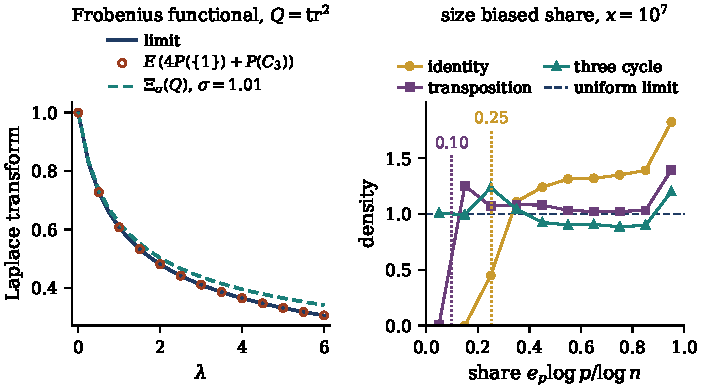
\includegraphics[width=\textwidth]{figs/pd_dirichlet.pdf}
\caption{Left: Theorem~\ref{thm:pddirichlet}(ii) for $Q=\operatorname{tr}^2$, the squared trace of the two dimensional representation of the $S_3$ field of $x^3-x-1$: the Laplace transform of the limit, $\exp(-\frac16\log(1+4\lambda)-\frac13\log(1+\lambda))$, that of two million samples of $E(4P(\{1\})+P(C_3))$, a standard exponential variable times a Dirichlet mean, and that of $\Xi_\sigma(Q)$ at $\sigma=1.01$ (primes below $10^7$, prime number theorem beyond). Right: the size biased share $e_p\log p/\log n$ of the $400000$ uniform random integers below $10^7$ of Figure~\ref{fig:pdintegers}, by Frobenius class of the chosen prime $p$. The limit is uniform for every class (Theorem~\ref{thm:pdsizebiased}); at $x=10^7$ the share is at least $\log59/\log10^7=0.25$ when $p$ is in the identity class, whose smallest prime is $59$, and at least $\log5/\log10^7=0.10$ when $p$ is in the class of transpositions, whose smallest prime is $5$ (both floors marked). The rise in the last bin is the atom at share $1$ of the prime powers $n=p^k$, nearly all of them primes.}\label{fig:pddirichlet}
\end{figure}

Theorem~\ref{thm:pddirichlet} has two readings. The first is Bayesian: in Chapter~\ref{ch:12} the Dirichlet process is a nonparametric prior on the trace law, set aside there because its draws are discrete; here it is the limit law of the labelled factorisation, with the equidistribution measure (Haar measure for Frobenius classes) as base measure, and Ferguson's conjugacy (\cite{ferguson1973}, Section~3, Theorem~1), which turns a prior with base measure $\vartheta\mu$ into a posterior with base measure $\vartheta\mu+\sum_i\delta_{y_i}$ after labels $y_1,\dots,y_n$, applies to it unchanged. The second is the Chinese restaurant process. Sampling points from a Dirichlet process with base measure $\vartheta\mu$ produces, by the P\'olya urn of Blackwell and MacQueen \cite{blackwellmacqueen1973}, a random partition: the $n$th point joins an existing cluster of size $m$ with probability $m/(n-1+\vartheta)$ and opens a new cluster, with a fresh label drawn from $\mu$, with probability $\vartheta/(n-1+\vartheta)$. The cluster sizes follow the Ewens sampling formula with parameter $\vartheta$ \cite{ewens1972,antoniak1974,hoppe1984}, and the cluster labels are independent with law $\mu$. For $\vartheta=1$ the partition of $n$ sampled points has the law of the cycle type of a uniform permutation of $n$ letters, which is the sense in which the large prime factors of a random integer and the long cycles of a random permutation have the same limit.

\section{The Ewens family from the coefficients of \texorpdfstring{$\zeta^\vartheta$}{zeta to the theta}}\label{sec:pdtheta}

The zeta subordinator $X_t$ of Chapter~\ref{ch:10d} runs, by Proposition~\ref{prop:10dsublaw}, through the random integers whose law is $d_t(n)n^{-\sigma}/\zeta(\sigma)^t$, where $d_t$ are the Dirichlet coefficients of $\zeta^t$, multiplicative with $d_t(p^k)=\binom{t+k-1}k$. For $t=1$ this is $N_\sigma$; for $t=2$ the weight is the divisor function. These integers, with $t=\vartheta$, give the whole Ewens family.

\begin{theorem}[the prime factors of the $\zeta^\vartheta$ random integer are Poisson Dirichlet with parameter $\vartheta$; after \cite{elboimgorodetsky2024,sun2026}]\label{thm:pdtheta}
Fix $\vartheta>0$ and let the random integer $N_\sigma^{(\vartheta)}$ have the law $d_\vartheta(n)n^{-\sigma}/\zeta(\sigma)^\vartheta$, with labels $(\theta_p)$ equidistributed with respect to $\mu$ outside $S$, and let $\Xi^{(\vartheta)}_\sigma=\sum_{p\notin S}(\sigma-1)e_p\log p\,\delta_{\theta_p}$ be its labelled factorisation. Then the prime exponents are independent negative binomial variables, $\Prob(e_p=k)=\binom{\vartheta+k-1}k(1-p^{-\sigma})^\vartheta p^{-k\sigma}$, and as $\sigma\downarrow1$:
\begin{enumerate}
\item[(i)] the marked process $\sum_{p\notin S,\,e_p\ge1}\delta_{((\sigma-1)e_p\log p,\,\theta_p)}$ converges in law, vaguely on $(0,\infty)\times Y$, to the Poisson process with intensity $\vartheta x^{-1}e^{-x}dx\otimes\mu$;
\item[(ii)] the labelled factorisation $\Xi^{(\vartheta)}_\sigma$ converges in law to the Gamma random measure with shape measure $\vartheta\mu$, its total mass, which is $(\sigma-1)\log N^{(\vartheta)}_\sigma$ up to the primes in $S$, to a Gamma variable with shape $\vartheta$, and the normalised factorisation to the Dirichlet process with base measure $\vartheta\mu$;
\item[(iii)] the ranked normalised sizes of the prime factors converge to $\mathrm{PD}(\vartheta)$, and for every continuous $Q\ge0$ the functional $\Xi^{(\vartheta)}_\sigma(Q)$ converges to a GGC with Thorin measure $\vartheta$ times the image of $\mu|_{\{Q>0\}}$ under $1/Q$.
\end{enumerate}
\end{theorem}

\begin{proof}
The generating function of the law is $\zeta(\sigma)^{-\vartheta}\sum_nd_\vartheta(n)n^{-\sigma}\prod_pt_p^{e_p}=\prod_p\bigl((1-p^{-\sigma})/(1-t_pp^{-\sigma})\bigr)^\vartheta$, a product over primes, so the exponents are independent and negative binomial. It is the $\vartheta$th power of the generating function of $N_\sigma$ (Lemma~\ref{lem:recipzeta}), so $\E e^{-\Xi^{(\vartheta)}_\sigma(\lambda)}=(\E e^{-\Xi_\sigma(\lambda)})^\vartheta$ for continuous $\lambda\ge0$, and Theorem~\ref{thm:recipgammaproc}(ii) gives the first two parts of (ii). The proof of Theorem~\ref{thm:recipgammaproc}(i) gives (i), with $\Prob(e_p=k)\le\binom{\vartheta+k-1}kp^{-k}$, whose sum over $k\ge2$ is $O(p^{-2})$, in place of $p^{-k}$, and $\vartheta p^{-\sigma}$ in place of $p^{-\sigma}$. The atoms of size below $a$ carry expected mass at most $\vartheta\nu_\sigma([0,a)\times Y)+O(\sigma-1)$, with $\nu_\sigma$ as in Lemma~\ref{lem:recipnu}, which tends to $\vartheta(1-e^{-a})$, uniformly small as $a\to0$; so the total mass converges jointly with the marked process of (i), and the ranked sizes divided by the total converge to the ranked jumps of a Gamma subordinator on $[0,\vartheta]$ divided by their sum, which is $\mathrm{PD}(\vartheta)$ \cite{kingman1975}. The third part of (ii) follows as in Theorem~\ref{thm:pddirichlet}, with $\Gamma_{\vartheta\mu}(Y)$ Gamma of shape $\vartheta$, and the GGC limit in (iii) is (ii) applied to $\lambda Q$, as in the proof of Theorem~\ref{thm:recipggcfun}.
\end{proof}

So the parameter of the Poisson Dirichlet law is the exponent $\vartheta$ of the singularity $(s-1)^{-\vartheta}$ of the generating Dirichlet series at $s=1$, the order of a pole when $\vartheta$ is an integer. For the Rankin Selberg random integer of an Artin representation $\rho$, with law proportional to the coefficients, which are nonnegative, of $L^S(s,\rho\otimes\check\rho)$, the $L$ function without its Euler factors at the ramified primes, the exponents are $e_p=\sum_mmM(p^m)$ with independent Poisson variables $M(p^m)$ of means $|\chi_\rho(\Frob_p^m)|^2p^{-m\sigma}/m$, and Theorem~\ref{thm:pdewens} below gives a marked limit with intensity $x^{-1}e^{-x}dx\otimes|\chi_\rho|^2\mu$, of total mass $\langle\rho,\rho\rangle$. So the Gamma shape of Theorem~\ref{thm:recipgamma} is an Ewens parameter, the normalised factorisation converges to the Dirichlet process with base measure $|\chi_\rho|^2\mu$ rather than a multiple of Haar measure, and the ranked sizes are $\mathrm{PD}(\langle\rho,\rho\rangle)$: $\mathrm{PD}(1)$ for irreducible $\rho$ and $\mathrm{PD}(4)$ for $\rho\oplus\rho$, with correspondingly more and smaller prime factors.

\section{Three colourings and their rates}\label{sec:pdmertens}

Theorem~\ref{thm:pddirichlet} is a statement about the zeta random integer as $\sigma\downarrow1$. For a uniform random integer below $x$ the sizes have the same limit (Theorem~\ref{thm:pdbillingsley}), but the rates differ sharply between three natural ways of colouring the prime factors by their Frobenius classes, and the differences are visible at $x=10^7$. Let $K/\Q$ be Galois with group $G$, $C\subset G$ a conjugacy class with Haar measure $\delta(C)=|C|/|G|$, which is $\mu(C)$ in the notation of Chapter~\ref{ch:recip}, and write $p\in C$ when the Frobenius class of $p$ is $C$. The three colourings of $n$ are: the class of the largest prime factor $P^+(n)$; the class of a \emph{size biased} prime factor, chosen with probability $e_p\log p/\log n$; and the classes of the distinct prime factors, pooled over $n$, that is the ratio $\E\omega_C(n)/\sum_{C'}\E\omega_{C'}(n)$, where $\omega_C(n)$ counts the distinct prime factors of $n$ in $C$.

\begin{theorem}[three colourings; (i) Dawsey \cite{dawsey2017}, (ii) this book, (iii) Mertens per class \cite{bardestanifreiberg2013}]\label{thm:pdmertens}
Let $n$ be uniform on $\{2,\dots,x\}$, and let the ramified primes be left out of every class. By the prime number theorem for $K$ in the form \cite{lagariasodlyzko1977}
\[
\pi_C(t)=\delta(C)\operatorname{li}(t)+O\bigl(t\exp(-a_K\sqrt{\log t})\bigr),
\]
the limits
\begin{align*}
b_C&=\lim_{t\to\infty}\Bigl(\sum_{p\le t,\,p\in C}\frac1p-\delta(C)\log\log t\Bigr),\\
c_C&=\lim_{t\to\infty}\Bigl(\sum_{p\le t,\,p\in C}\frac{\log p}p-\delta(C)\log t\Bigr)
\end{align*}
exist, with $\sum_Cb_C=B-\sum_{p\text{ ram.}}1/p$ and $\sum_Cc_C=c-\sum_{p\text{ ram.}}\log p/p$, where $B=0.26150$ and $c=-\gamma_{\mathrm E}-\sum_p\log p/(p(p-1))=-1.33258$ are the two Mertens constants. Let $\kappa_C=-c_C-\sum_{p\in C}\log p/(p(p-1))$, which by the Abelian theorem is the Euler Kronecker drift of Theorem~\ref{thm:recipdrift} for $S$ the set of ramified primes, so that $\sum_C(\gamma_{\mathrm E}\delta(C)-\kappa_C)=-\sum_{p\text{ ram.}}\log p/(p-1)$. Then, as $x\to\infty$:
\begin{enumerate}
\item[(i)] $\Prob(P^+(n)\in C)=\delta(C)+O\bigl(\exp(-a_K'(\log x)^{1/3})\bigr)$ for some $a_K'>0$;
\item[(ii)] the size biased prime factor lies in $C$ with probability
\[
\delta(C)+\frac{\gamma_{\mathrm E}\delta(C)-\kappa_C}{\log x-1}+O\bigl((\log x)^{-2}\bigr);
\]
\item[(iii)] $\E\,\omega_C(n)=\delta(C)\log\log x+b_C+O(1/\log x)$, so that with $B'=B-\sum_{p\text{ ram.}}1/p$ the ratio of means $\E\omega_C(n)/\sum_{C'}\E\omega_{C'}(n)$, the share of the unramified distinct prime factors that lie in $C$, equals
\[
\delta(C)+\frac{b_C-\delta(C)B'}{\log\log x+B'}+O\Bigl(\frac1{\log x\,\log\log x}\Bigr).
\]
\end{enumerate}
\end{theorem}

\begin{proof}
The constants exist by partial summation against $\pi_C(t)-\delta(C)\operatorname{li}(t)$, exactly as in Mertens's theorems for $\pi(t)$ \cite{mertens1874,tenenbaum2015}; the sums over all classes are the classical constants. (i) is Dawsey's theorem (\cite{dawsey2017}, Theorem~2), which extends Alladi's for progressions \cite{alladi1977}. The error is so small because the unlabelled count is exact: every $n$ with $2\le n\le x$ is $pm$ with $p=P^+(n)$ and $m\le x/p$ free of primes above $p$, so $\sum_{p\le x}\Psi(x/p,p)=\lfloor x\rfloor-1$, with $\Psi(y,p)$ the number of such $m\le y$, and only the equidistribution of the primes of $C$, weighted by $\Psi(x/p,p)$, enters. (iii) By Mertens's theorem for the class (\cite{bardestanifreiberg2013}, Theorems~8.3 and 8.5),
\begin{align*}
\E\omega_C(n)&=\frac1{\lfloor x\rfloor-1}\sum_{p\le x,\,p\in C}\Bigl\lfloor\frac xp\Bigr\rfloor=\sum_{p\le x,\,p\in C}\frac1p+O\Bigl(\frac1{\log x}\Bigr)\\
&=\delta(C)\log\log x+b_C+O\Bigl(\frac1{\log x}\Bigr);
\end{align*}
summing over the classes gives $\log\log x+B'+O(1/\log x)$, and the ratio of the two expansions is the display. (ii) Write $\ell_C(n)=\sum_{p\in C}e_p\log p$, so that the size biased factor lies in $C$ with probability $\E[\ell_C(n)/\log n]$. Replacing $1/\log n$ by $1/(\log x-1)$, where $\log x-1+O(\log x/x)$ is the mean of $\log n$, costs $O((\log x)^{-2})$: for $n\ge\sqrt x$, writing $u=\log(n/x)$,
\[
\frac1{\log n}=\frac1{\log x-1}-\frac{u+1}{(\log x-1)^2}+O\Bigl(\frac{(u+1)^2}{(\log x)^3}\Bigr);
\]
the first order term is handled by $\E[\ell_C(n)(u+1)]=O(1)$, because for each prime power $y=x/p^k$ the inner sum $\sum_{m\le y}(\log(m/y)+1)$ is $O(\log y+1)$, the second by $\E[\ell_C(n)(u+1)^2]\le\log x\,\E(u+1)^2=O(\log x)$, and the $n<\sqrt x$ have probability $O(x^{-1/2})$. Now $(\lfloor x\rfloor-1)\E e_p=\sum_{k\ge1}\lfloor x/p^k\rfloor=x/(p-1)-\sum_{k\ge1}\{x/p^k\}$. Summing over $p\le x$ in $C$, with $x/(\lfloor x\rfloor-1)=1+O(1/x)$, the main term is
\[
\sum_{p\le x,\,p\in C}\frac{\log p}{p-1}=\delta(C)\log x+c_C+\sum_{p\in C}\frac{\log p}{p(p-1)}+O\Bigl(\frac1{\log x}\Bigr)
\]
by the definition of $c_C$, and the fractional parts contribute
\[
-\frac1x\sum_{p\le x,\,p\in C}\log p\,\Bigl\{\frac xp\Bigr\}+O\Bigl(\frac1{\log x}\Bigr)=-\delta(C)(1-\gamma_{\mathrm E})+O\Bigl(\frac1{\log x}\Bigr).
\]
The last estimate is the class version of
\[
\sum_{n\le x}\Lambda(n)\Bigl\{\frac xn\Bigr\}=(1-\gamma_{\mathrm E})x+O\Bigl(\frac x{\log x}\Bigr),
\]
which follows from $\log\lfloor x\rfloor!=\sum_{n\le x}\Lambda(n)\lfloor x/n\rfloor$ and $\sum_{n\le x}\Lambda(n)/n=\log x-\gamma_{\mathrm E}+o(1/\log x)$: on each interval $x/(j+1)<p\le x/j$ with $j<\log x$ the function $\{x/p\}=x/p-j$ is monotone, and partial summation against $\sum_{p\le t,\,p\in C}\log p-\delta(C)\sum_{p\le t}\log p=O(t\exp(-a_K\sqrt{\log t}))$ replaces the sum over $p\in C$ by $\delta(C)$ times the sum over all primes, with an error $O(x/\log x)$, the primes $p\le x/\log x$ contributing $O(x/\log x)$. This term $-\delta(C)(1-\gamma_{\mathrm E})$ is why the constant carries the term $\gamma_{\mathrm E}\delta(C)$. Hence $\E\ell_C(n)=\delta(C)(\log x-1)+\gamma_{\mathrm E}\delta(C)-\kappa_C+O(1/\log x)$, and dividing by $\log x-1$ gives (ii).
\end{proof}

For the zeta integer the same constant is, by Theorem~\ref{thm:recipdrift}, the first order term of the ratio of means $\E L_C(\sigma)/\E[(\sigma-1)\log N_\sigma]=\delta(C)+(\gamma_{\mathrm E}\delta(C)-\kappa_C)(\sigma-1)+O((\sigma-1)^2)$, with $L_C(\sigma)$ the rescaled class mass of Corollary~\ref{cor:recipchebgamma} and $\sigma-1$ in the place of $1/(\log x-1)$.

\begin{table}[!htbp]
\centering\small
\begin{tabular}{@{}lccccc@{}}
\toprule
class $C$ of $x^3-x-1$ & $\delta(C)$ & $b_C$ & $c_C$ & $\gamma_{\mathrm E}\delta(C)-\kappa_C$ & smallest prime\\
\midrule
identity ($3$ roots) & $1/6$ & $-0.2436$ & $-0.7429$ & $-0.6439$ & $59$\\
transposition ($1$ root) & $1/2$ & $-0.0755$ & $-0.5931$ & $-0.1211$ & $5$\\
three cycle ($0$ roots) & $1/3$ & $0.5372$ & $-0.1327$ & $0.6226$ & $2$\\
\bottomrule
\end{tabular}
\caption{Mertens constants per Frobenius class, computed from the unramified primes below $10^7$, for the $S_3$ extension of $x^3-x-1$; the ramified prime $23$ is left out, so the $b_C$ sum to $0.2180=B-\frac1{23}$ and the $c_C$ to $-1.4687$, against the limit $c-\frac{\log23}{23}=-1.4689$. The identity class has a large negative $b_C$ because its first prime is $59$; the three cycle class, which contains $2$, $3$ and $13$, has a large positive one.}\label{tab:pdmertens}
\end{table}

Table~\ref{tab:pdmertens} gives the constants for the running example, and Figure~\ref{fig:pdintegers}, bottom, compares the three colourings at $x=10^7$ with Haar measure and with the predictions of the theorem. The largest prime factor is already close to Haar: shares $0.161$, $0.506$, $0.332$ against $\frac16,\frac12,\frac13$, the deviation at this $x$ coming from the small primes. For the zeta integer this is Theorem~\ref{thm:hitrate}(ii), and Chapter~\ref{ch:hit} computes its approach, linear in $\sigma-1$, for the same field. The size biased factor has shares $0.124$, $0.492$, $0.374$, against the prediction $0.124$, $0.492$, $0.375$ of (ii), and the remaining $0.93$ percent of picks fall on the ramified prime $23$, against $\log23/(22(\log x-1))$, that is $0.94$ percent. The distinct prime factors, pooled over all $400000$ integers, have shares $0.072$, $0.438$, $0.489$, against the prediction $0.073$, $0.438$, $0.488$ of (iii), and the identity class is at less than half its Haar measure. The reason is in the last column of the table: the count of distinct prime factors is dominated by small primes, whose classes are fixed, and the identity class has no prime below $59$. The deficit of its share, $(b_C-\delta(C)B')/(\log\log x+B')$ with $b_C-\delta(C)B'=-0.280$, decays only like $1/\log\log x$: it is $-0.093$ at $x=10^7$ and still $-0.059$ at $x=10^{40}$. Chebotarev's theorem holds for all three colourings, but for the third the identity class is still more than a third below its Haar measure at $x=10^{40}$. The same effect sits inside Theorem~\ref{thm:pdsizebiased} below: the Frobenius class and the size of a size biased factor are asymptotically independent, but at $x=10^7$ a size biased factor in the identity class carries at least $\log59/\log10^7=0.25$ of $\log n$ (Figure~\ref{fig:pddirichlet}, right). So the statistics of a random integer that see Chebotarev's theorem at a computable scale are those that select or weight prime factors by their size, as the Frobenius functionals of Chapter~\ref{ch:recip} do with the weight $e_p\log p$; counting distinct prime factors, where the small primes dominate, does not.

\begin{theorem}[size biased factors are uniform, whatever their class; after Donnelly and Grimmett \cite{donnellygrimmett1993}]\label{thm:pdsizebiased}
Let $n$ be uniform on $\{2,\dots,x\}$, let $p^*$ be a size biased prime factor of $n$, and let $F^*=e_{p^*}\log p^*/\log n$ be its share. As $x\to\infty$, $p^*$ is unramified with probability tending to $1$, and $(F^*,\text{class of }p^*)$ converges in law to the product of the uniform law on $(0,1)$ and the law $C\mapsto\delta(C)$ on the classes. The same holds for the zeta random integer as $\sigma\downarrow1$, with $p^*$ picked, off $A_\sigma$, among the prime factors outside $S$ and its share taken relative to their part of $\log N_\sigma$.
\end{theorem}

\begin{proof}
For the uniform integer the statement is a first moment computation:
\[
\Prob(p^*\in C,\ F^*\le f)=\E\sum_{p\in C}\frac{e_p\log p}{\log n}\mathsf1\{e_p\log p\le f\log n\}.
\]
The terms with $e_p\ge2$ contribute $O(1/\log x)$, the integers $n\le x/(\log x)^2$ contribute $O((\log x)^{-2})$, and for the others $\log n=\log x+O(\log\log x)$, so the probability is $(\log x)^{-1}\sum_{p\le x^f,\,p\in C}\log p/p+O(\log\log x/\log x)=\delta(C)f+o(1)$ by Mertens's first theorem for the class, which follows from the existence of $c_C$ in Theorem~\ref{thm:pdmertens}. For the zeta integer, the proof of Theorem~\ref{thm:pdtheta} with $\vartheta=1$ shows that the rescaled sizes with their labels and the total mass converge jointly, so that the normalised sizes converge to $\mathrm{PD}(1)$, a limit that goes back to Lloyd \cite{lloyd1984}, with labels independent of the sizes and of law $\mu$ (Theorem~\ref{thm:recipgammaproc}(i)). Since picking in proportion to size is a continuous operation outside a null set, the share of $p^*$ converges to a size biased pick from $\mathrm{PD}(1)$, which is uniform (\cite{pitman2006}, Section~3.1), and its class to an independent label of law $\mu$.
\end{proof}

\section[Mertens constants, empty classes and Ewens parameters]{Mertens constants, empty classes\\ and Ewens parameters}\label{sec:pdprogress}

This section answers two questions about the limits above and bounds a third from one side. The Mertens constants per class are explicit in $L(1,\chi)$ and $\frac{L'}L(1,\chi)$ (Theorem~\ref{thm:pdmertensL}). The Ewens parameter of an Euler product whose logarithm has nonnegative coefficients, given at the primes by a continuous function of equidistributed labels, is the exponent of its singularity at $s=1$, the order of its pole when it continues meromorphically, and the colouring of its random integer is the equidistribution measure weighted by that function (Theorem~\ref{thm:pdewens}). And while the Euler Kronecker drifts of Chapter~\ref{ch:recip} govern the means, the Kolmogorov distance between the law of the share of a class $C$ and its Beta limit is at least of order $(\sigma-1)^{\delta(C)}$, because at any $\sigma>1$ the class is empty with probability of that order, which Chapter~\ref{ch:recip} found (Theorem~\ref{thm:recipggcfun} and the paragraph after it) and Theorem~\ref{thm:pdrate} gives with its constant. The constants of the first and last answers come from one function, the regular part $h_C$ of the partial Euler product over a class: $b_C$ and the constant of the last answer from its value at $s=1$, and $c_C$ from its derivative there.

Throughout, $K/\Q$ is Galois with group $G$, $S$ is the set of ramified primes and $C$ a class with $\delta(C)=|C|/|G|$. As in the proof of Theorem~\ref{thm:recipdrift},
\[
P_C(s)=\sum_{p\notin S,\ \Frob_p\in C}\ \sum_{m\ge1}\frac{p^{-ms}}m=\sum_\chi c_\chi\log L^S(s,\chi)+R_C(s),
\]
with $c_\chi=\delta(C)\overline{\chi(C)}$ for each irreducible character $\chi$, $L^S$ the $L$ function without its Euler factors at $S$, and a prime power term $R_C$ holomorphic on $\operatorname{Re}s>\frac12$. By Brauer's theorem and the nonvanishing of Artin $L$ functions at $s=1$, $h_C(s)=P_C(s)-\delta(C)\log\frac1{s-1}$ is real analytic near $s=1$, and $h_C'(1)$ is the drift $\kappa_C$ of that theorem for this $S$.

\subsection{Mertens constants from \texorpdfstring{$L(1,\chi)$}{L(1,chi)}}

\begin{theorem}[Mertens constants per class; after \cite{williams1974,bardestanifreiberg2013}]\label{thm:pdmertensL}
With $b_C$ and $c_C$ as in Theorem~\ref{thm:pdmertens} and $B$, $c$ the Mertens constants,
\begin{align*}
b_C&=\delta(C)\Bigl(B-\sum_{p\in S}\frac1p\Bigr)+\sum_{\chi\ne1}c_\chi\Bigl[\log L^S(1,\chi)-\sum_{p\notin S}\sum_{m\ge2}\frac{\chi(\Frob_p^m)}{m\,p^m}\Bigr],\\
c_C&=\delta(C)\Bigl(c-\sum_{p\in S}\frac{\log p}p\Bigr)-\sum_{\chi\ne1}c_\chi\Bigl[\frac{(L^S)'}{L^S}(1,\chi)+\sum_{p\notin S}\sum_{m\ge2}\frac{\chi(\Frob_p^m)\log p}{p^m}\Bigr],
\end{align*}
and the constant term of $P_C$ at $s=1$ is
\[
h_C(1)=b_C-\gamma_{\mathrm E}\,\delta(C)+\sum_{p\notin S,\,\Frob_p\in C}\ \sum_{m\ge2}\frac{p^{-m}}m .
\]
\end{theorem}

\begin{proof}
Expand $\mathsf1_C(\Frob_p)=\sum_\chi c_\chi\chi(\Frob_p)$. The term $\chi=1$ gives, by Mertens, $\delta(C)$ times $\sum_{p\le t,\,p\notin S}1/p$, which is $\log\log t+B-\sum_{p\in S}1/p+o(1)$. For $\chi\ne1$ the partial sums $\sum_{p\le t,\,p\notin S}\chi(\Frob_p)/p$ converge to the bracket in the theorem: the Dirichlet series $\sum_{p\notin S}\chi(\Frob_p)p^{-s}$ equals $\log L^S(s,\chi)$ minus the prime power sum, which is holomorphic on $\operatorname{Re}s>\frac12$, and $L^S(s,\chi)$ is holomorphic and nonzero on $\operatorname{Re}s\ge1$, so the partial sums converge to the value at $s=1$ by the prime number theorem for $K$ and partial summation, exactly as for Dirichlet characters \cite{tenenbaum2015}; for Chebotarev classes see \cite{bardestanifreiberg2013}, Theorem~8.3. The formula for $c_C$ is the same argument with $\log p/p$ in place of $1/p$, the $\chi=1$ term being the prime number theorem in the form $\sum_{p\le t}\log p/p=\log t+c+o(1)$ and the others the derivative of $-\log L^S(s,\chi)$ at $1$. For $h_C(1)$, the Abelian theorem $\sum_{p\in C}p^{-s}=\delta(C)\log\frac1{s-1}+b_C-\gamma_{\mathrm E}\delta(C)+o(1)$ follows from $\sum_{p\le t,\,p\in C}1/p=\delta(C)\log\log t+b_C+o(1)$ by partial summation, and the prime powers add their convergent sum.
\end{proof}

The formula for $c_C$ is Theorem~\ref{thm:recipdrift} in other terms: by the Abelian theorem $c_C+\sum_{p\in C}\log p/(p(p-1))=-\kappa_C$, minus the drift of the class $C$. The formula for $b_C$, its analogue for the weights $1/p$ with $\log L(1,\chi)$ in place of $\frac{L'}L(1,\chi)$, is (8.1), (8.2) and Theorem~8.3 of Bardestani and Freiberg \cite{bardestanifreiberg2013}, and the asymptotic $\prod_{p\le x,\,p\in C}(1-1/p)\sim e^{-h_C(1)-\gamma_{\mathrm E}\delta(C)}(\log x)^{-\delta(C)}$ is (8.8) of the same theorem, and with an error term Theorem~A of Arango Pi\~neros, Keliher and Keyes \cite{arangopinerokeliherkeyes2022}.

For the $S_3$ field of $x^3-x-1$, with $S=\{23\}$, the characters are the trivial one, the sign $\chi_{-23}$ and the two dimensional $\rho$, with $L(1,\chi_{-23})=3\pi/\sqrt{23}=1.965202$, $L^{(23)}(1,\rho)=0.352392$, $\frac{L'}L(1,\chi_{-23})=-0.422121$ and $\frac{(L^{(23)})'}{L^{(23)}}(1,\rho)=1.159587$ from PARI. The theorem gives $b_C=-0.243641$, $-0.075520$, $0.537179$ and $c_C=-0.742978$, $-0.593191$, $-0.132738$ for the identity, the transpositions and the three cycles, against the values $-0.243638$, $-0.075516$, $0.537183$ and $-0.742913$, $-0.593134$, $-0.132674$ read from the primes below $10^7$ in Table~\ref{tab:pdmertens}; the differences, below $7\cdot10^{-5}$, are the tails beyond $10^7$, and with the primes below $10^9$ they fall below $3\cdot10^{-5}$. The constants $h_C(1)$ are $-0.33954$, $-0.32024$ and $0.61533$. What the theorem leaves open is the sign of the deficit of the identity class as the field varies, Open Problem~\ref{op:pdmertens}.

\subsection{Atoms at zero: a class is empty with probability of order \texorpdfstring{$(\sigma-1)^{\delta(C)}$}{(sigma-1) to the delta(C)}}

For $Q=\mathsf1_C$ the probability in Theorem~\ref{thm:recipggcfun} that no prime factor of $N_\sigma$ has a label where $Q>0$ is the probability that the class $C$ is empty, of exact order $(\sigma-1)^{\delta(C)}$ by the paragraph after that theorem. The next theorem gives its constant, and the atom at zero that it describes bounds from below the Kolmogorov distance between the law of a share and its Beta limit.

\begin{theorem}[atoms at zero and a lower bound for the rate; (i) refines Theorem~\ref{thm:recipggcfun}, (iii) after Serre \cite{serre1976}]\label{thm:pdrate}
Let $G$ be nontrivial, let $L_C(\sigma)$ be the mass of the class $C$, as in Corollary~\ref{cor:recipchebgamma}, let $A_\sigma$ be the event that $N_\sigma$ has no prime factor outside $S$, and let $\mathcal P_\sigma(C)$ be the share of $C$, equal to $L_C(\sigma)/\sum_{C'}L_{C'}(\sigma)$ off $A_\sigma$ and to $\delta(C)$ on $A_\sigma$, as in Theorem~\ref{thm:pddirichlet}.
\begin{enumerate}
\item[(i)] $\Prob(L_C(\sigma)=0)=e^{-P_C(\sigma)}=e^{-h_C(1)}(\sigma-1)^{\delta(C)}\bigl(1+O(\sigma-1)\bigr)$, with $h_C(1)$ as in Theorem~\ref{thm:pdmertensL}.
\item[(ii)] The Kolmogorov distance between the law of $\mathcal P_\sigma(C)$ and its limit $\mathrm{Beta}(\delta(C),1-\delta(C))$ is at least
\[
\Prob(L_C(\sigma)=0)-\Prob(A_\sigma)=e^{-h_C(1)}(\sigma-1)^{\delta(C)}\bigl(1+o(1)\bigr),
\]
hence at least of order $(\sigma-1)^{\delta_{\min}}$ for the smallest class, $\delta_{\min}=\min_C\delta(C)$.
\item[(iii)] For the uniform random integer below $x$ the same exponent appears in the density of the integers free of $C$: the proportion of $n\le x$ with no prime factor in $C$ equals $K_C(\log x)^{-\delta(C)}(1+O(1/\log x))$, where
\[
K_C=\frac{e^{\gamma_{\mathrm E}\delta(C)}}{\Gamma(1-\delta(C))}\lim_{t\to\infty}(\log t)^{\delta(C)}\prod_{p\le t,\,p\in C}\Bigl(1-\frac1p\Bigr)=\frac{e^{-h_C(1)}}{\Gamma(1-\delta(C))}:
\]
the same constant $e^{-h_C(1)}$ governs the zeta integer, through $e^{-h_C(1)}(\sigma-1)^{\delta(C)}$, and the uniform integer, through $e^{-h_C(1)}(\log x)^{-\delta(C)}/\Gamma(1-\delta(C))$.
\end{enumerate}
\end{theorem}

\begin{proof}
(i) By Lemma~\ref{lem:recipzeta} the exponents are independent and $\Prob(e_p=0)=1-p^{-\sigma}$, so $\Prob(L_C(\sigma)=0)=\prod_{p\in C}(1-p^{-\sigma})=\exp(-P_C(\sigma))$, and $P_C(\sigma)=\delta(C)\log\frac1{\sigma-1}+h_C(1)+O(\sigma-1)$ by the analyticity of $h_C$. (ii) The Beta law has no atom at $0$, while $\mathcal P_\sigma(C)=0$ exactly when $L_C(\sigma)=0$ and $A_\sigma$ fails, and $A_\sigma\subset\{L_C(\sigma)=0\}$; the distribution functions therefore differ at $0$ by $\Prob(L_C(\sigma)=0)-\Prob(A_\sigma)$, and $\Prob(A_\sigma)=\prod_{p\notin S}(1-p^{-\sigma})=O(\sigma-1)$, which is $o((\sigma-1)^{\delta(C)})$ because $\delta(C)<1$. (iii) is a case of Serre's theorem on frobenian sets \cite{serre1976}, proved by Landau's method \cite{landau1908}, which gives an expansion in powers of $1/\log x$; Wirsing's theorem \cite{wirsing1961} gives its leading term without the rate. For the multiplicative indicator $f$ of the integers free of primes in $C$, whose mean value over the primes is $1-\delta$, with $\delta=\delta(C)$, Wirsing's theorem reads
\[
\sum_{n\le x}f(n)\sim\frac{e^{-\gamma_{\mathrm E}(1-\delta)}\,x}{\Gamma(1-\delta)\log x}\prod_{p\le x,\,p\notin C}\Bigl(1-\frac1p\Bigr)^{-1},
\]
and Mertens's third theorem turns the product into $e^{\gamma_{\mathrm E}}\log x\prod_{p\le x,\,p\in C}(1-1/p)$. The second form of $K_C$ follows from Theorem~\ref{thm:pdmertensL}, which gives
\[
\sum_{p\le t,\,p\in C}\log\Bigl(1-\frac1p\Bigr)=-\delta\log\log t-h_C(1)-\gamma_{\mathrm E}\delta+o(1).\qedhere
\]
\end{proof}

In the Kolmogorov distance of the shares the theorem gives a lower bound of order $(\sigma-1)^{\delta_{\min}}$, far above the order $(\sigma-1)\log\frac1{\sigma-1}$ at which the means converge (below); the matching upper bound is Open Problem~\ref{op:pdrate}. For the $S_3$ field, $\delta_{\min}=\frac16$, and the identity class, the primes that split completely, is empty with probability $0.647$, $0.444$ and $0.303$ at $\sigma=1.01$, $1.001$ and $1.0001$, against $0.652$, $0.444$ and $0.303$ from (i) with $h_C(1)=-0.33954$; the transpositions are empty with probability $0.137$, $0.044$, $0.014$ and the three cycles with probability $0.117$, $0.054$, $0.025$. At $\sigma=1.0001$ the Kolmogorov distance between the law of the share of the identity class and its Beta limit is still at least $0.30$. Since $\mathrm{Beta}(\delta,1-\delta)$ puts mass about $\varepsilon^\delta\sin(\pi\delta)/(\pi\delta)$ on $[0,\varepsilon]$, the same atom forces only a L\'evy distance of order $\sigma-1$, about $10^{-3}$ at $\sigma=1.0001$. The means behave differently. The share means $\E[\mathcal P_\sigma(C);\,A_\sigma^c]$, computed as $\int_0^\infty(-\phi_C')\prod_{C'\ne C}\phi_{C'}\,dt$ from the Laplace transforms $\phi_C(t)=\E e^{-tL_C(\sigma)}$, are $0.1427$, $0.4871$, $0.3599$ at $\sigma=1.01$ and $0.1628$, $0.4986$, $0.3375$ at $\sigma=1.001$. For the identity class they fall short of $\delta(C)(1-\Prob(A_\sigma))$, the value the mean would have if the shares were exactly Dirichlet off $A_\sigma$, by $0.022$ and $0.0037$. The deficit has an exact form: since $\phi_C(t)=e^{P_C(s)-P_C(\sigma)}$ with $s=\sigma+t(\sigma-1)$, by Lemma~\ref{lem:recipzeta}, it equals $(\sigma-1)\int_\sigma^\infty(h_C'(s)-\delta(C)h'(s))e^{h(s)-h(\sigma)}\,ds/(s-1)$ with $h=\sum_{C'}h_{C'}$, which is $(\kappa_C-\delta(C)\sum_{C'}\kappa_{C'})(\sigma-1)\log\frac1{\sigma-1}+O(\sigma-1)$, the drifts of Theorem~\ref{thm:recipdrift} entering through $h_C'(1)=\kappa_C$; for the identity class the coefficient is $0.620$. So the Euler Kronecker constants govern the convergence of the means, and the constants $h_C(1)$ govern the atom at zero, which keeps the Kolmogorov distance of the shares at least of order $(\sigma-1)^{\delta(C)}$.

The exponent is the same one that governs the counting function of the uniform integers: the number of integers below $x$ with no prime factor in $C$ is of order $x(\log x)^{-\delta(C)}$, which for the inert primes of $\Q(i)$ is the order $x/\sqrt{\log x}$ of Landau's count of sums of two squares \cite{landau1908}. Among the $400000$ integers below $10^7$ of Section~\ref{sec:pdmertens}, $79.3$ percent have no prime factor in the identity class, $19.8$ percent none among the transpositions and $15.7$ percent none among the three cycles; and the asymptotic of (iii) with the constants $K_C=e^{-h_C(1)}/\Gamma(1-\delta(C))$ gives $78.3$, $19.4$ and $15.8$ percent, the remaining gaps, $1.1$, $0.4$ and $-0.1$ points, being of the size of the $1/\log x$ term at $\log x=16.1$.

\subsection{The Ewens parameter of an \texorpdfstring{$L$}{L} function}

\begin{theorem}[Ewens parameters are pole orders; after \cite{arratiakochmanmiller2014,elboimgorodetsky2024}]\label{thm:pdewens}
Let $D(s)=\sum_na(n)n^{-s}=\exp\bigl(\sum_p\sum_{m\ge1}w_m(p)p^{-ms}/m\bigr)$ be an Euler product with $w_m(p)\ge0$ bounded, and suppose the labels $(\theta_p)$ are equidistributed with respect to $\mu$ on the compact space $Y$ and $w_1(p)=w(\theta_p)$ outside a finite set of primes, for a continuous $w\ge0$ on $Y$ with $\int w\,d\mu>0$. Let $N^D_\sigma$ have the law $a(n)n^{-\sigma}/D(\sigma)$, $\sigma>1$. Then the prime exponents of $N^D_\sigma$ are independent, $e_p=\sum_mmM(p^m)$ with independent Poisson variables of means $w_m(p)p^{-m\sigma}/m$, and as $\sigma\downarrow1$ the labelled factorisation converges in law to the Gamma random measure with shape measure $w\mu$, the normalised factorisation to the Dirichlet process with base measure $w\mu$, and the ranked normalised sizes to $\mathrm{PD}(\vartheta)$ with
\[
\vartheta=\int_Yw\,d\mu=\lim_{s\downarrow1}\frac{\log D(s)}{\log\frac1{s-1}},
\]
the order of the pole of $D$ at $s=1$ when $D$ continues meromorphically. In particular: for $D=L(s,\rho\otimes\check\rho)$, $w=|\chi_\rho|^2$ and $\vartheta=\langle\rho,\rho\rangle$, the Gamma shape of Theorem~\ref{thm:recipgamma}; for $D=\zeta_K$ with $K/\Q$ of degree $n$ and Galois closure of group $G$ acting on the $n$ embeddings, $w(g)$ is the number of fixed points of $g$ and $\vartheta=1$ by Burnside's lemma.
\end{theorem}

\begin{proof}
The generating function of the exponents factorises over primes as $\prod_p\exp(\sum_mw_m(p)p^{-m\sigma}(t_p^m-1)/m)$, which is the Poisson representation. The proof of Theorem~\ref{thm:recipgammaproc} uses only this structure and Lemma~\ref{lem:recipnu} with the weights $w_1(p)$: the measure $(\sigma-1)\sum_pw(\theta_p)(\log p)p^{-\sigma}\delta_{((\sigma-1)\log p,\,\theta_p)}$ converges to $e^{-x}dx\otimes w\mu$ because $w$ is continuous and $(\theta_p)$ is equidistributed, and the prime powers $m\ge2$ contribute a bounded expected number of atoms, of total expected rescaled mass $O(\sigma-1)$, which vanish in the limit. The rest is Theorem~\ref{thm:pddirichlet} with $\mu$ replaced by $w\mu$ and the Gamma total mass of shape $\int w\,d\mu$, and the ranked sizes follow as in the proof of Theorem~\ref{thm:pdtheta}, with the intensity $x^{-1}e^{-x}dx\otimes w\mu$ in place of $\vartheta x^{-1}e^{-x}dx\otimes\mu$. The identification of $\vartheta$ with the pole order extends Lemma~\ref{lem:recipvirtual}, which gives it for Artin $L$ functions: $\log D(s)=\sum_pw(\theta_p)p^{-s}+O(1)$ and $\sum_pw(\theta_p)p^{-s}=(\int w\,d\mu+o(1))\log\frac1{s-1}$ by equidistribution and partial summation, which is all the limit needs. For $\rho\otimes\check\rho$ the coefficients $w_m(p)=|\chi_\rho(\Frob_p^m)|^2$ are nonnegative (at a ramified prime, the average of $|\chi_\rho|^2$ over the inertia coset); for $\zeta_K$ the Euler factor at $p$ is $\prod_i(1-p^{-f_is})^{-1}$ over the primes above $p$, so $w_m(p)=\sum_{f_i\mid m}f_i$ is the number of fixed points of $\Frob_p^m$ on the embeddings, and $\int w\,d\mu=1$ is Burnside's count of orbits.
\end{proof}

Theorem~\ref{thm:pdtheta} is the case $w_m(p)=\vartheta$, that is $D=\zeta^\vartheta$. Theorem~\ref{thm:pdewens} also says something the unlabelled theory does not: the colouring of the Rankin Selberg integer is not Haar measure but $|\chi_\rho|^2\mu$. For the two dimensional representation of $S_3$, $|\chi_\rho|^2$ is $4$, $0$, $1$ on the identity, the transpositions and the three cycles, so the base measure puts mass $\frac23$ on the identity and $\frac13$ on the three cycles: primes with Frobenius a transposition occur in the Rankin Selberg integer only to even powers, and their share tends to zero. We checked this on the Laplace transforms of the three class masses, computed from the primes below $10^7$ with the prime number theorem for the tail: at $\sigma=1.001$ and $\lambda=4$ they are $0.346$, $0.9975$ and $0.583$ against the limits $(1+\lambda)^{-2/3}=0.342$, $1$ and $(1+\lambda)^{-1/3}=0.585$.

\section{Discussion: what Bondesson's theory contributes}\label{sec:pdbondesson}

The generalized gamma convolutions were introduced by Thorin \cite{thorin1977,thorin1977b} to prove that the Pareto and lognormal laws are infinitely divisible, and the theory was built by Bondesson \cite{bondesson1992}. The structure theorem (an infinitely divisible law on $[0,\infty)$ is a GGC if and only if its L\'evy density is $k(x)/x$ with $k$ completely monotone, equivalently $-\varphi'/\varphi$ is a Stieltjes function with no pole at the origin, integrable at $0$), self decomposability, unimodality and closure under convolution and weak limits were recalled after Definitions~\ref{def:ch10ggc} and \ref{def:10bstieltjes} (unimodality of self decomposable laws is Yamazato's theorem \cite{yamazato1978}), and Stieltjes inversion is Theorem~\ref{thm:lapstieltjes}. Since much of Part IV takes place in this class, it is worth saying which further results of Bondesson do arithmetic work here and which do not.

\emph{Mass and shape.} If the drift vanishes and the Thorin mass $m=\tau((0,\infty))$ is finite, the density is $f(x)=x^{m-1}g(x)/\Gamma(m)$ with $g$ completely monotone and $g(0+)=\exp\int\log t\,\tau(dt)$, finite when $\int_1^\infty\log t\,\tau(dt)<\infty$, for instance when $\tau$ has bounded support; in every case $m=\sup\{\alpha:f(x)x^{1-\alpha}\to0\text{ as }x\downarrow0\}$ is the exponent of small values (\cite{bondesson1992}, Chapter~4; \cite{jamesroynetteyor2008}, Section~1.3). If moreover $m\le1$, the density is completely monotone, that is the law is a mixture of exponential laws. The Thorin mass of a Frobenius functional is $\mu(Q>0)$ (Theorem~\ref{thm:recipggcfun}), and the atom at zero of Theorem~\ref{thm:pdrate}, of order $(\sigma-1)^{\delta(C)}$, has the same exponent as the small values of the limit law, $m=\delta(C)$; the order of the pole of $L(s,\rho\otimes\check\rho)$ at $s=1$ is the Thorin mass of the Gamma limit of Theorem~\ref{thm:recipgamma} and the Ewens parameter of Theorem~\ref{thm:pdewens}. Every class has $\delta(C)\le1$, so the limit law $\mathrm{Gamma}(\delta(C))$ of the mass $L_C$ of a Chebotarev class is a mixture of exponentials, and its normalisation is the Beta law of Theorem~\ref{thm:pddirichlet}; only when $\langle\rho,\rho\rangle\ge2$, that is for reducible $\rho$, does the Gamma limit of Theorem~\ref{thm:recipgamma} leave the mixtures of exponentials, and the loss of complete monotonicity is a probabilistic reading of reducibility.

\emph{Hyperbolic complete monotonicity.} A density $f$ on $(0,\infty)$ is HCM if, for every $u>0$, the function $f(uv)f(u/v)$ is completely monotone as a function of $v+1/v$. Every HCM law is a GGC; the HCM class is closed under products, quotients and powers $x^q$, $|q|\ge1$, of independent variables; and it contains the gamma, lognormal and beta of the second kind laws (\cite{bondesson1992}, Chapter~5) and the positive stable laws of index at most $\frac12$ \cite{boschsimon2016}. This book does not use it. The factorisation of a GGC of finite Thorin mass as a Gamma variable times an independent Dirichlet mean, in Section~\ref{sec:pddirichlet} and Theorem~\ref{thm:lapspline}, is Cifarelli and Regazzini's identity \cite{cifarelliregazzini1990} and holds for every Dirichlet mean; HCM variables enter it through Bondesson's theorem that a Gamma variable times an independent HCM variable is a GGC, which makes every HCM variable with a finite negative moment of order $m$ a Dirichlet mean (\cite{jamesroynetteyor2008}, Proposition~1.5). Whether the Thorin variable of Theorem~\ref{thm:laptail} is HCM is not known to us.

\emph{Closure and arithmetic.} Multiplying $L$ functions, that is taking direct or isobaric sums, convolves the corresponding laws and adds Thorin measures. The passage $\sigma\downarrow1$ does not come from closure under weak limits: at $\sigma>1$ a Frobenius functional is a compound Poisson law with an atom at $0$, not a GGC (\cite{sato1999}, Section~27), and its GGC limit, with Thorin measure the image of Haar measure restricted to $\{Q>0\}$ under $1/Q$, comes from the Poisson structure of the prime exponents (Theorem~\ref{thm:recipgammaproc}). By a later theorem of Bondesson \cite{bondesson2015} the product of two independent GGC variables is again a GGC; this multiplicative closure has no arithmetic counterpart that we know of, and Open Problem~\ref{op:pdproduct} asks for one. The prime side need not stay in the class under the operations of the Langlands programme: the sine squared lemma (Lemma~\ref{lem:10dsin2}) turns a L\'evy measure into a Thorin density when the logarithmic coefficients are nonnegative, as for $L(s,\pi\times\tilde\pi)$, a sufficient condition and not a necessary one; symmetric powers and base change have signed coefficients in general, their transported densities can be signed (Section~\ref{sec:10daway}), and the Thorin representation of such an $L$ function to the right of its zeros comes from its Hadamard product (Theorem~\ref{thm:10dshift}), that is from its automorphy.

\emph{The limits.} Bondesson's theorems are structural, not arithmetic. They translate conjectures and theorems (GRH into membership of the class, Theorem~\ref{thm:10bmain}; irreducibility into Thorin mass one; Chebotarev's theorem into the base measure of a Dirichlet process), but they do not produce the automorphic partner of a Galois representation or the Galois partner of an automorphic one. For a self dual automorphic $\pi$ the Thorin measure at a basepoint $\frac12+a$ with $a\ge\frac12$ exists whatever the zeros, each zero $\beta+i\gamma$ entering through Cauchy noise of scale $a-\beta$ (Theorem~\ref{thm:lapcauchy}), and at $a=0$ its existence is GRH. For an Artin representation $\rho$ the Thorin representation at a basepoint $\alpha>1$ is unconditional when the logarithmic coefficients are nonnegative, as for $\rho\otimes\check\rho$ (Proposition~\ref{prop:recipfamily}); for $\rho$ itself (with $\check\rho$ when $\rho$ is not self dual) it is known when $\rho$ is automorphic (Theorem~\ref{thm:10dshift}(iii)), and at the centre it is the holomorphy of $\Lambda(s,\rho)$ together with GRH, for self dual $\rho$ the complete monotonicity of the Galois heat trace (Theorem~\ref{thm:recipcm}). The Thorin measures of a Galois representation and of an automorphic representation are each computable to any precision, and reciprocity is the assertion that they coincide, which no closure property will supply. What the theory supplies is a class of positive objects in which the two sides can be compared.

\subsection{Open problems}

\begin{problem}[The upper bound for the rate]\label{op:pdrate}
Theorem~\ref{thm:pdrate} shows that, in the Kolmogorov distance of the shares, the Dirichlet process limit is approached no faster than $(\sigma-1)^{\delta_{\min}}$. Prove the matching upper bound: that the Kolmogorov distance between the law of $\mathcal P_\sigma(C)$ and $\mathrm{Beta}(\delta(C),1-\delta(C))$ is $O((\sigma-1)^{\delta(C)})$, and that, for the Euclidean distance between share vectors, the Wasserstein distance between the laws of $(\mathcal P_\sigma(C))_C$ and of its Dirichlet limit is $O((\sigma-1)\log\frac1{\sigma-1})$, the order at which the means converge.
\end{problem}

\begin{problem}[Signs of the Mertens deficits]\label{op:pdmertens}
Theorem~\ref{thm:pdmertensL} expresses $b_C$ and $c_C$ through $L(1,\chi)$ and $\frac{L'}L(1,\chi)$. For the splitting field of a polynomial of degree $n$ with group $S_n$, the deficit of the identity class in Theorem~\ref{thm:pdmertens}(iii) is $b_{\{1\}}-\delta(\{1\})B'=\lim_{t\to\infty}\sum_{p\le t,\,p\notin S}(\mathsf1_{\{1\}}(\Frob_p)-\delta(\{1\}))/p$; it is $-0.280$ for $x^3-x-1$, whose smallest completely split prime is $59$. A prime $p<n$ splits completely only if it divides the index of $\Z[\alpha]$, with $\alpha$ a root of the polynomial, and this happens: in Dedekind's field of $x^3-x^2-2x-8$ the prime $2$ splits completely and adds $\frac5{12}$ to the sum. Read from the primes below $10^7$, the deficit is $0.224$ for Dedekind's field and $0.245$ for $x^3-x+15$, in which $3$ and $5$ split completely, so both signs occur already with group $S_3$. Determine the distribution of the sign of the deficit over the fields with group $S_n$ ordered by discriminant, and its sign along a family such as $x^n-x-1$. This is the analogue, for the weights $1/p$, of Open Problem~\ref{op:recipdrift}; Problem 24.2 computes the constants.
\end{problem}

\begin{problem}[An arithmetic product]\label{op:pdproduct}
By Bondesson \cite{bondesson2015} the product of two independent GGC variables is a GGC, so the product of independent copies of the limits of $\Xi_\sigma(Q_1)$ and $\Xi_\sigma(Q_2)$ in Theorem~\ref{thm:recipggcfun} is a GGC, with a Thorin measure $\tau_{Q_1,Q_2}$. Multiplying Dirichlet series realises the additive closure, the Frobenius functional of the product of two independent random integers being the sum of two independent ones, and tensor products, as in Rankin Selberg convolution, give the functional of $Q_1Q_2$. Find the arithmetic operation, if any, that realises the multiplicative closure: a representation or an $L$ function whose Frobenius functional has Thorin measure $\tau_{Q_1,Q_2}$; and compute $\tau_{Q_1,Q_2}$ for $Q_1=Q_2=\operatorname{tr}^2$ on $S_3$. For a finite group the Thorin measure of a limiting Frobenius functional is finitely supported and that of such a product is not, so the operation, if any, leads to an infinite label space, such as a Sato Tate group.
\end{problem}

\section{Notes}

The Poisson Dirichlet law is Kingman's \cite{kingman1975}, and the Gamma process description is in his book (\cite{kingman1993}, Chapter~9). For permutations the limit goes back to Shepp and Lloyd \cite{shepplloyd1966}; for prime factorisations it is Billingsley's theorem \cite{billingsley1972}, found independently by Knuth and Trabb Pardo \cite{knuthtrabbpardo1976}, and Tenenbaum \cite{tenenbaum2000} proved the rate $1/\log x$ as an expansion in powers of $1/\log x$ whose term in $1/\log x$ is, for each prime factor separately, Knuth and Trabb Pardo's. Donnelly and Grimmett \cite{donnellygrimmett1993} proved Billingsley's theorem by size biased sampling, which gives the uniform share of Theorem~\ref{thm:pdsizebiased}; Arratia, Barbour and Tavar\'e \cite{arratiabarbourtavare2003} treat integers and permutations together; Pitman's lectures \cite{pitman2006} cover stick breaking, size biased sampling, the GEM law and the Chinese restaurant process (Sections~3.1, 3.2 and 4.1). The route through the zeta random integer is Lloyd's \cite{lloyd1984}, as recalled in Chapter~\ref{ch:recip}.

Dickman's function is from \cite{dickman1930}, the Erd\H{o}s Kac theorem from \cite{erdoskac1940}, the Sathe Selberg formula from \cite{sathe1953,selberg1954}, and the variance of $\omega(n)$ with its constant from Diaconis, Mosteller and Onishi \cite{diaconismostelleronishi1977}. Mertens's theorems are in \cite{mertens1874}, which already treats arithmetic progressions; for progressions the constants are in Williams \cite{williams1974} and Languasco and Zaccagnini \cite{languascozaccagnini2007}. For a Chebotarev class, Bardestani and Freiberg (\cite{bardestanifreiberg2013}, Section~8, Theorem~8.3) give $b_C$ in the form of Theorem~\ref{thm:pdmertensL}, and Arango Pi\~neros, Keliher and Keyes (\cite{arangopinerokeliherkeyes2022}, Theorem~A) give the asymptotic of $\prod_{p\le x,\,p\in C}(1-1/p)$ with an error term; the expression of $c_C$ through $\frac{L'}L(1,\chi)$ is the drift of Theorem~\ref{thm:recipdrift}. Dawsey (\cite{dawsey2017}, Theorem~2) proved that the class of the largest prime factor is equidistributed with error $O(\exp(-a_K'(\log x)^{1/3}))$, extending Alladi's theorem for progressions \cite{alladi1977}; this is Theorem~\ref{thm:pdmertens}(i). The counts $\omega_C(n)$ are asymptotically independent Poisson variables with means $\delta(C)\log\log x+b_C$ (Delange \cite{delange1971}, Section~6.5.3, for two classes; Tenenbaum \cite{tenenbaum2017}, for any number of classes, with a rate; see Ford \cite{ford2022}), which refines Theorem~\ref{thm:pdmertens}(iii). The density of the integers free of the primes of a class, with an expansion in powers of $1/\log x$ and the constant $K_C$, is a case of Serre's theorem on frobenian sets \cite{serre1976}, proved by Landau's method \cite{landau1908}; Odoni \cite{odoni1975} treated norms, and Wirsing's theorem \cite{wirsing1961} gives the asymptotic without the rate.

The Dirichlet process is Ferguson's (\cite{ferguson1973}, Section~3, Theorem~1, for the posterior and Section~4 for the normalised Gamma process); the urn for its samples is Blackwell and MacQueen's \cite{blackwellmacqueen1973}, and the Ewens sampling formula \cite{ewens1972} for its clusters is due to Antoniak \cite{antoniak1974}, with Hoppe's urn \cite{hoppe1984}. The identity $\E(1+\lambda\int Q\,dP)^{-\vartheta}=\exp(-\vartheta\int\log(1+\lambda Q)\,d\mu)$ for the means of a Dirichlet process with base measure $\vartheta\mu$ is Cifarelli and Regazzini's \cite{cifarelliregazzini1990}, the Markov Krein identity when $\vartheta=1$ (Diaconis and Kemperman \cite{diaconiskemperman1996}, Corollary~2 and Section~3), in the form of James, Roynette and Yor (\cite{jamesroynetteyor2008}, Section~1.4, (33)) that Theorem~\ref{thm:lapspline} uses. For integers weighted by $d_\vartheta(n)$, and more generally by multiplicative weights of mean $\vartheta$ on the primes, the Poisson Dirichlet law with parameter $\vartheta$ is due to Elboim and Gorodetsky, who also prove the Erd\H{o}s Kac law with mean and variance $\vartheta\log\log x$ in this generality (\cite{elboimgorodetsky2024}, Theorem~1.1; for weights bounded on the primes, such as $d_\vartheta$, that law is in \cite{tenenbaum2017}, Corollary~2.5), and for normed arithmetic semigroups whose primes have density $\vartheta$, such as the integers composed of primes in a set of progressions or the Gaussian integers counted by norm, the Poisson Dirichlet law is due to Arratia, Kochman and Miller (\cite{arratiakochmanmiller2014}, Theorem~2 and Section~5). For the $\zeta^\vartheta$ random integer itself, the unlabelled limits of Theorem~\ref{thm:pdtheta} are Sun's (\cite{sun2026}, Propositions~4.2 and 4.3).

The generalized gamma convolutions are Thorin's \cite{thorin1977,thorin1977b}; Bondesson's monograph \cite{bondesson1992} has the structure, density and HCM results recalled in Section~\ref{sec:pdbondesson} (Chapters~3 to 5), and the product closure is \cite{bondesson2015}. Self decomposable laws are unimodal by Yamazato's theorem \cite{yamazato1978}, and the positive stable law of index $\alpha$ is HCM if and only if $\alpha\le\frac12$ (Bosch and Simon \cite{boschsimon2016}).

What is ours, as far as we know, is the labelled form at $\sigma\downarrow1$: the normalised labelled factorisation of the zeta random integer converges to the Dirichlet process with base measure $\mu$, Haar measure for Frobenius labels (Theorem~\ref{thm:pddirichlet}, whose part (iii) for finitely many labels is Corollary~\ref{cor:recipchebgamma}(ii)), with its versions for the $\zeta^\vartheta$ integer and for Euler products whose logarithm has nonnegative coefficients, of base measures $\vartheta\mu$ and $w\mu$ (Theorems~\ref{thm:pdtheta} and \ref{thm:pdewens}); the expansion of the size biased colouring with the constant $\gamma_{\mathrm E}\delta(C)-\kappa_C$ (Theorem~\ref{thm:pdmertens}(ii)) and the independence of class and share (Theorem~\ref{thm:pdsizebiased}); and the reading of the classical constant $e^{-h_C(1)}$ as the atom at zero of the zeta integer, whose order is that of Theorem~\ref{thm:recipggcfun}, with the Kolmogorov bound it gives (Theorem~\ref{thm:pdrate}(i) and (ii)). Each follows from Theorem~\ref{thm:recipgammaproc}, Ferguson's construction and the theorems above, and through them everything known about $\mathrm{PD}(\vartheta)$, the Ewens sampling formula and Dirichlet means applies to the Frobenius labelled factorisations of Chapter~\ref{ch:recip}.

\section{Exercises}

\begin{enumerate}
\item Show that the stick breaking sequence $W_k=(1-U_1)\cdots(1-U_{k-1})U_k$ has $\E W_k=2^{-k}$, $\E W_k^2=3^{-k}$ and $\sum_k\E W_k^2=\frac12$. Deduce $\E\sum_kV_k^2=\frac12$ for $\mathrm{PD}(1)$, the case $\vartheta=1$ of $1/(1+\vartheta)$, and check it on the random integers of Section~\ref{sec:pdlaw}.
\item Compute Dickman's $\varrho$ on $[1,3]$ from its delay equation and verify $\varrho(2)=1-\log2=0.30685$ and $\varrho(3)=0.04861$.
\item Show that for a Dirichlet process $P$ with base measure $\mu$ on the conjugacy classes of a finite group and $Q=\mathsf1_C$ the Dirichlet mean $\int Q\,dP$ is $\mathrm{Beta}(\mu(C),1-\mu(C))$, and that $E\int Q\,dP$, with $E$ standard exponential and independent of $P$, is then Gamma with shape $\mu(C)$; compare with Corollary~\ref{cor:recipchebgamma}(i).
\item Derive the Ewens sampling formula with parameter $\vartheta$ from the Chinese restaurant process, and show that for $\vartheta=1$ it gives the law of the cycle type of a uniform permutation.
\item Prove that $\sum_Cc_C=c-\sum_{p\text{ ram.}}\log p/p$, which is $-1.4689$ for $x^3-x-1$, where $c=\lim(\sum_{p\le t}\log p/p-\log t)=-\gamma_{\mathrm E}-\sum_p\log p/(p(p-1))=-1.33258$, and compute $\sum_p\log p/(p(p-1))$ to six digits.
\item For the Rankin Selberg random integer of $\rho\oplus\rho$, with $\vartheta=4$, simulate the ranked normalised prime factors at $\sigma=1.01$ and compare the mean of the largest with the $\mathrm{PD}(4)$ value (for $\mathrm{PD}(\vartheta)$, $\E V_1=\vartheta^{-1}\int_0^\infty(1-e^{-\vartheta E_1(x)})\,dx$, with $E_1(x)=\int_x^\infty e^{-t}t^{-1}dt$).
\item Show that the number of prime factors of $N_\sigma^{(\vartheta)}$ counted with multiplicity has mean $\vartheta\sum_pp^{-\sigma}/(1-p^{-\sigma})$ and is asymptotically normal as $\sigma\downarrow1$ with mean and variance $\vartheta\log\frac1{\sigma-1}$; this is the Erd\H{o}s Kac theorem for the Ewens family.
\end{enumerate}

\section{Open computational problems}

The scripts named below are in \texttt{pd/code/} (Section~\ref{sec:B:scripts}).

\begin{compproblem}[Colourings at scale]\label{cp:pdcolour}
Objective: for uniform random integers below $x$, compute the three colourings of Theorem~\ref{thm:pdmertens} (the class of the largest prime factor, the class of a size biased prime factor, and the pooled classes of the distinct prime factors) and the proportion of integers with no prime factor in each class, and compare them with the predictions: Haar measure up to Dawsey's error $O(\exp(-a_K'(\log x)^{1/3}))$ for the largest factor, Theorem~\ref{thm:pdmertens}(ii) and (iii) for the other two and Theorem~\ref{thm:pdrate}(iii) for the proportions, with the constants computed through Theorem~\ref{thm:pdmertensL}. Objects and scale: the $S_3$ field of $x^3-x-1$, the $S_4$ field of $x^4-x-1$, and as an abelian control the cyclic cubic field of conductor $7$; $10^6$ integers at each of $x=10^9$, $10^{12}$ and $10^{15}$. Route: \texttt{pd1.py} and \texttt{pd2.py}, with the sieve replaced by \texttt{factorint} in PARI/GP for the sampled integers; the class of a prime $p$ is the factorisation pattern of the polynomial modulo $p$ (\texttt{factormod}), which determines it in $S_3$ and $S_4$, and $p\bmod7$ in the cyclic field; $L(1,\chi)$ and $\frac{L'}L(1,\chi)$ from Dedekind zeta functions of subfields (\texttt{lfuncreate} and \texttt{lfundiv}, as \texttt{op\_pd.py} does for $S_3$), checked against prime sums to $10^9$. Deliverable: for each field, class and $x$, the three shares and the proportions of integers with an empty class, with binomial standard errors, against the predictions with and without their second order terms, and the scale at which each colouring is within one standard error of Haar measure. Why it matters: at $x=10^7$ the distinct prime factors put the identity class of $x^3-x-1$ at less than half its Haar measure, and Theorem~\ref{thm:pdmertens}(iii) says the deficit decays only like $1/\log\log x$; the table shows how much of Chebotarev's theorem each colouring sees at computable scales, and the identity class of the $S_4$ field, of Haar measure $\frac1{24}$, is a sharper test than that of $S_3$.
\end{compproblem}

\begin{compproblem}[Mertens constants of symmetric fields]\label{cp:pdsn}
Objective: compute the Mertens constants $b_C$ and $c_C$ of Theorem~\ref{thm:pdmertens} and the constants $h_C(1)$ and $K_C$ of Theorem~\ref{thm:pdrate} for every class of the splitting field of $x^n-x-1$, and determine the sign of the deficit $b_{\{1\}}-\delta(\{1\})B'$ of the identity class that Open Problem~\ref{op:pdmertens} asks about. Objects and scale: $3\le n\le7$; primes up to $10^{10}$. Route: confirm with \texttt{polgalois} that the group is $S_n$; form the partial sums over the primes up to $10^{10}$ by a segmented sieve, each prime not dividing the discriminant of $x^n-x-1$ classed by the factorisation pattern of $x^n-x-1$ modulo $p$, which is its cycle type and so determines its class in $S_n$, and the other unramified primes by \texttt{idealprimedec}; take the tail beyond $10^{10}$ from the prime number theorem for the field, with an error estimate under GRH; for $n\le5$ obtain an independent value through Theorem~\ref{thm:pdmertensL}, the characters of $S_n$ being integer combinations of the permutation characters of Young subgroups (Young's rule), whose $L$ functions are Dedekind zeta functions of subfields of the splitting field (\texttt{lfuncreate} and \texttt{lfundiv} in PARI/GP). Deliverable: tables of $b_C$, $c_C$, $h_C(1)$ and $K_C$ for all classes with error estimates, the two routes compared where both apply, and the deficit of the identity class against $n$. Why it matters: Open Problem~\ref{op:pdmertens} rests on $S_3$ alone, and Problem 20.3, which computes drifts of Galois fields of degree at most $10$, does not reach the splitting fields of degree $24$ and more. The deficit is $-0.280$ for $x^3-x-1$, whose first completely split prime is $59$, while a completely split prime $p$ adds $(1-\delta(\{1\}))/p$ to the sum that defines it, $\frac5{12}$ for the prime $2$ of Dedekind's field in Open Problem~\ref{op:pdmertens}; so its sign along $x^n-x-1$ is the question.
\end{compproblem}

\begin{compproblem}[Laws of class shares near $\sigma=1$]\label{cp:pdshares}
Objective: compute the laws of the class masses $L_C(\sigma)$ of the zeta random integer and of the shares $\mathcal P_\sigma(C)$, the Kolmogorov distance of each share from its limit $\mathrm{Beta}(\delta(C),1-\delta(C))$, and the means of the shares, and fit the rates in $\sigma-1$ that Theorem~\ref{thm:pdrate} and Open Problem~\ref{op:pdrate} concern. Objects and scale: the $S_3$ field of $x^3-x-1$ and the $S_4$ field of $x^4-x-1$; $10^{-5}\le\sigma-1\le10^{-1}$. Route: the Laplace transforms $\E e^{-tL_C(\sigma)}$ from the Euler products over the primes up to $10^{10}$ and the prime number theorem for the field beyond, or from the $L$ functions through the decomposition of $P_C$ at the start of Section~\ref{sec:pdprogress}, as \texttt{op\_pd.py} does; off $A_\sigma$ the event $\mathcal P_\sigma(C)\le u$ is $(1-u)L_C(\sigma)\le u\sum_{C'\ne C}L_{C'}(\sigma)$, whose probability follows by Gil Pelaez inversion of characteristic functions, checked by Monte Carlo at $\sigma-1=10^{-2}$. Deliverable: for each class, the Kolmogorov distance and the defect of the mean against $\sigma-1$ on log log axes, with fitted exponents and constants, compared with $e^{-h_C(1)}(\sigma-1)^{\delta(C)}$ for the distance and $(\sigma-1)\log\frac1{\sigma-1}$ for the means. Why it matters: Theorem~\ref{thm:pdrate} proves the lower bound only; a fitted exponent equal to $\delta(C)$ with a constant near $e^{-h_C(1)}$, and a defect of the means of order $(\sigma-1)\log\frac1{\sigma-1}$, are the numerical content of Open Problem~\ref{op:pdrate}, which the zero probability exponents of Problem 20.3 do not decide.
\end{compproblem}
